\documentclass{article}
\usepackage[utf8]{inputenc}

\title{Assignment-7\\Synchronization}
\author{Subash Mylraj \\(CED18I051) }
\date{30 November 2020}

\usepackage{geometry}
 \geometry{
 a4paper,
 total={170mm,257mm},
 left=20mm,
 top=10mm,
 }

\usepackage{longtable}
\usepackage{graphicx}
\usepackage{listings}
\usepackage{xcolor}

\begin{document}

\maketitle

\lstset{
  language=c,
  aboveskip=3mm,
  belowskip=3mm,
  showstringspaces=false,
  columns=flexible,
  basicstyle={\small\ttfamily},
  numbers=none,
  numberstyle=\tiny\color{gray},
  keywordstyle=\color{blue},
  commentstyle=\color{dkgreen},
  stringstyle=\color{mauve},
  breaklines=true,
  breakatwhitespace=true,
  tabsize=3
}

\definecolor{dkgreen}{rgb}{0,0.6,0}
\definecolor{gray}{rgb}{0.5,0.5,0.5}
\definecolor{mauve}{rgb}{0.58,0,0.82}

\section*{Question 1: Simulate the Producer Consumer code discussed in the class.}
\bigskip

\par\noindent
\textbf{\Large Code: }
\smallskip
\par\noindent\rule{\textwidth}{0.4pt}
\lstinputlisting[language=c]{src/1.c}
\par\noindent\rule{\textwidth}{0.4pt}

\bigskip
\noindent
\textbf{\Large Explanation: } \\

This program is a simulation of a solution to the producer consumer problem.
This solution uses a circular queue, where the producer produces until the queue
is full and the consumer consumes until the queue is empty. Once the queue is full, 
the consumer stops producing.

\bigskip
\noindent
\textbf{\Large Output:}

\begin{figure}[h]
	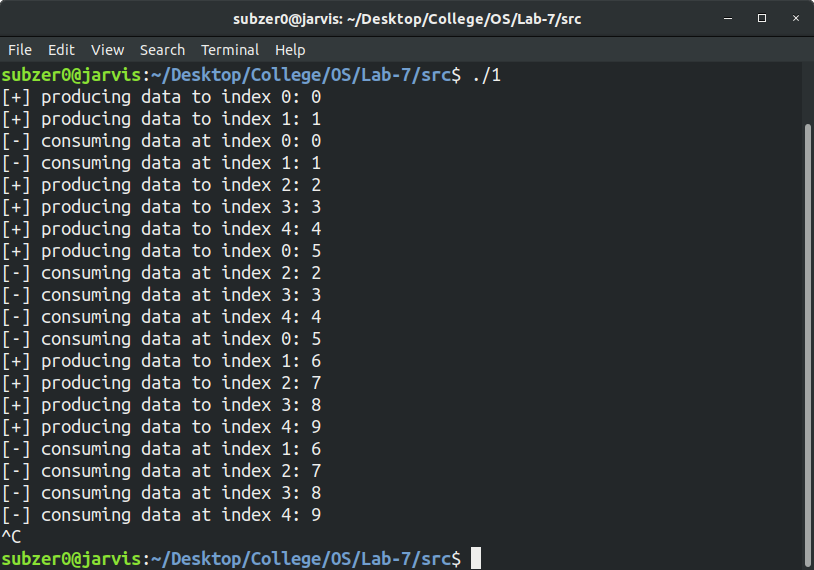
\includegraphics[width=\textwidth]{output/1.png}
\end{figure}
\bigskip

\section*{Question 2: Extend the producer consumer simulation in Q1 to sync access of critical data using Petersons algorithm.}
\bigskip

\par\noindent
\textbf{\Large Code: }
\smallskip
\par\noindent\rule{\textwidth}{0.4pt}
\lstinputlisting[language=c]{src/2.c}
\par\noindent\rule{\textwidth}{0.4pt}

\bigskip
\noindent
\textbf{\Large Explanation: } \\

This program is an extension to the previous program. Petersons algorithm is used to attain
synchronization between the producer and the consumer. The variable counter is used to keep
track of the status of the buffer. If it is full, then the producer does not produce anything.
If it is empty, then the consumer does not consume anything.


\bigskip
\noindent
\textbf{\Large Output:}

\begin{figure}[h]
	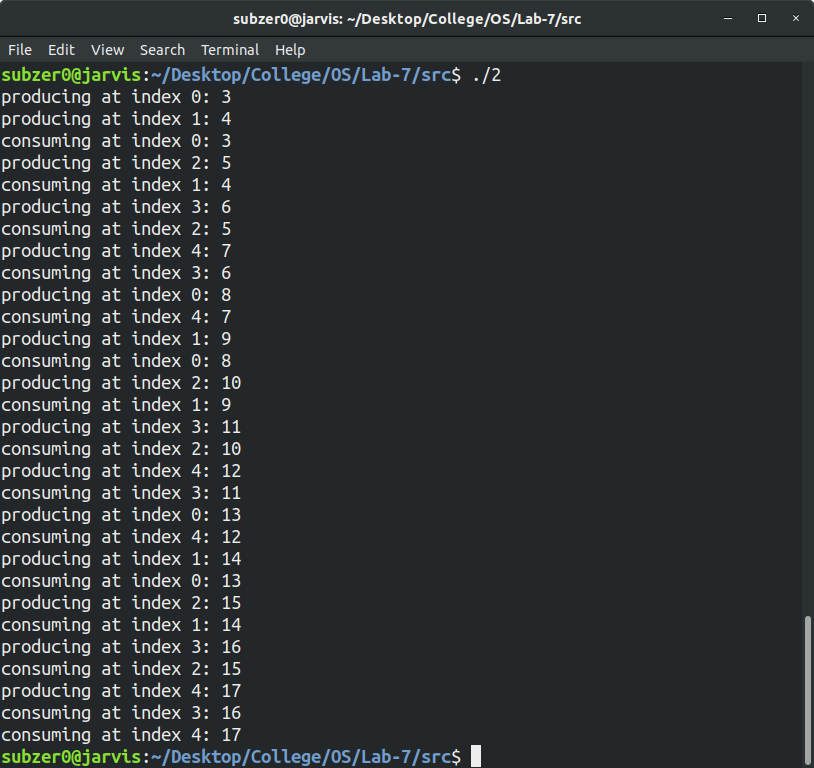
\includegraphics[width=\textwidth]{output/2.png}
\end{figure}
\bigskip
\pagebreak

\section*{Question 3: Dictionary Problem: Let the producer set up a dictionary of at least 20 words with three attributes (Word, Primary meaning, Secondary meaning) and let the consumer search for the word and retrieve its respective primary and secondary meaning.}
\bigskip

\par\noindent
\textbf{\Large Code: }
\smallskip
\par\noindent\rule{\textwidth}{0.4pt}
\lstinputlisting[language=c]{src/3.c}
\par\noindent\rule{\textwidth}{0.4pt}
\bigskip

\par\noindent
\textbf{\Large Dictionary: }
\smallskip
\par\noindent\rule{\textwidth}{0.4pt}
\lstinputlisting[language=c]{src/dict.txt}
\par\noindent\rule{\textwidth}{0.4pt}

\bigskip
\noindent
\textbf{\Large Explanation: } \\

dict.txt contains a list of words with 2 of its meanings. This file contains the data in csv format (comma separated values).
This program searches for a word in this list. The producer parses the file and puts the word structure in the buffer.
The consumer pulls the words from the buffer and checks whether the pulled word is the key. 

\bigskip
\noindent
\textbf{\Large Output:}

\begin{figure}[h]
	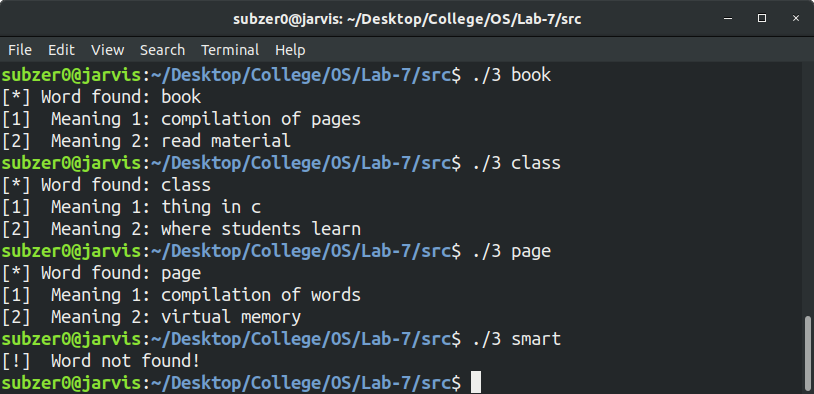
\includegraphics[width=\textwidth]{output/3.png}
\end{figure}
\bigskip


\end{document}